\section{Обзор литературы}

\subsection{Решения задачи в общем случае}

\begin{enumerate}
    \item $\O(n^3 k^3)$ \cite{Reps97}

    Грамматика приводится к Нормальной форме Хомского, считается $dp_{i,j,c}$~--- выводится ли путь $i \path j$ из нетерминала $s$, при добавлении 1 ($dp_{i,j,A} = 1$) перебираются все соседние нетерминалы $B$, т.ч. $\exists C \to AB$ (или $C \to BA$) и $k \in V(G)$, и если $dp_{j, k, B}$ (или $dp_{k, i, B}$), то $dp_{i, k, C} = 1$ (или $dp_{k, j, C} = 1$) и $(i, k, C)$ добавляется в рабочую очередь.

    \item $\O(n^3 k^3 / \log n)$ \cite{Chaudhuri08}

    Алгоритм \cite{Reps97}, к которому применили метод 4 русских

\end{enumerate}

\subsection{Решения задачи в частных случаях}

Понятно, что для решения практических задач далеко не всегда нужна CFPQ в общем случае. Чаще всего для каждой конкретной задачи нужна конкретная КС грамматика, а иногда ещё и понятны ограничения на тип графа.

Пользуясь этой информацией (ограничениями на тип грамматики и графа) можно конструировать частные и потому более быстрые решения. Этим уже занимались, сейчас мы выпишем всё, что на текущий момент известно:

\begin{enumerate}
    \item Язык Дика $\O(n^3 k)$ \cite{Kodumal04}

    Просто применить алгоритм Репса \cite{Reps97} и нормально оценить время работы.

    \item Язык Дика (почти) $\O(n^3)$ \cite{Rehof01}

    Ещё более точный анализ алгоритм Репса \cite{Reps97}, учитывающий, что построенный (для конкретного анализа) граф содержит константное число скобок

    \item Язык Дика на одном типе скобок $D_1$ $\O(n^{\omega} \log^2 n)$ \cite{Mathiasen21}

    \begin{definition}[Bell-shaped путь]
        Путь, который понимается строго вверх, потом сколько-то идёт ровно ($\eps$-рёбра), потом спускается строго вниз
    \end{definition}

    Ищем bell-shaped пути: удваиваем рёбра, ищем пути с серединкой из bell-shaped пути поменьше (так $\log n^2$ раз).

    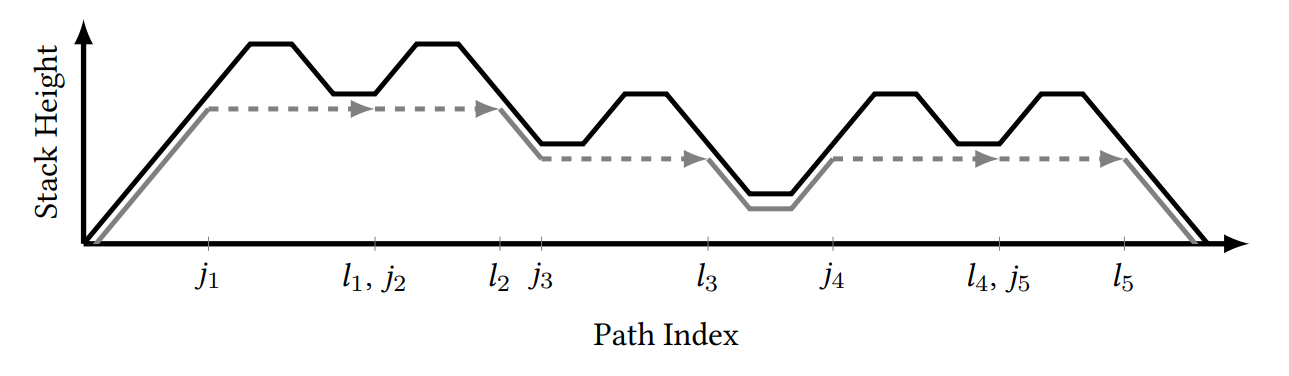
\includegraphics[width=0.75\linewidth]{img/dyck1_path.png}

    Сжимаем bell-shaped пути в $\eps$-рёбра. Снова ищем и снова сжимаем. После каждого сжимания мы убираем все локальные максимумы. Чем больше был максимум, тем длиннее $\eps$-ребро. Хуже всего, когда все новые рёбра длины 2. В любом случае путь становится короче хотя бы в 2 раза, так что таких итераций потребуется не более $\log n^2$ (есть лемма, что найдётся путь длины не более $\O(n^2)$). 

    \item Двунаправленные графы и язык Дика

    Существует несколько частных решений для задачи Диковой достижимости на двунаправленных графах:

    \begin{itemize}
        \item Деревья \cite{Yuan09}

        $\O(n \log n \log k)$~--- центроиды + внутри что-то идейное

        \item Общий случай \cite{Chatterjee17}

        Решение основано на двух фактах. Первый: в двунаправленном графе формируются компоненты Диковой достижимости. Второй: если есть две вершины $u, v$ и компонента Диковой достижимости $C$, такие что $u \xrightarrow{\alpha_i} C$ и $v \xrightarrow{\alpha_i} C$, то $u$ и $v$ тоже лежат в одной компоненте Диковой достижимости. 

        Пользуясь этими фактами, алгоритм с помощью СНМ'а поддерживает компоненты Диковой достижимости и исходящие из них рёбра, чтобы быстро искать новые пары вершин, принадлежащих одной компоненте.

        Итоговая асимптотика алгоритма $\O(m + n \alpha(n))$.

        \item Interleaved Dyck reachability

        Алгоритм за $\O(n^7)$ для $D_1 \bigodot D_1$ достижимости на bidirected графах: 
        \url{https://helloqirun.github.io/papers/popl21_yuanbo.pdf}

        Было ещё про это (там, вроде, про один из языков сказали, что он bounded, поэтому можно пересекать с регулярным): 
        \url{https://dl.acm.org/doi/pdf/10.1145/3296979.3192378}
    \end{itemize}

    \item Граф-цепочка $\O(n^{\omega})$ \cite{Valiant1975}

        CFPQ на графе-цепочке~--- просто задача КС-распознавания (CF-recognition). А она решается за перемножение булевых матриц \cite{Valiant1975}

    \item Ацикличный граф $\O(n^{\omega})$ \cite{Yannakakis1990}

        Ацикличный граф~--- это почти бамбук (= цепочка), нужно только его потопсорить (и где-то ещё быть аккуратным, я не совсем помню сведение)

    \item Bounded-stack RSM $\O(n^3 k^3 / \log^2)$ \cite{Chaudhuri08}

        RSM, который не уходит в рекурсию (т.е. есть из конца ребра $\xrightarrow{S}$ не достижимо никакое ребро $\xrightarrow{S}$)

        Тут применяется какое-то более хитрое (я ещё не разбиралась) итеративное транзитивное замыкание (что-то с dfs'ом, а потом ещё 4 русских сверху, кажется)

    \item Hierarchical FSM $\O(n^{\omega} k^{\omega})$ \cite{Chaudhuri08}

        RSM, в котором боксы упорядочены (топсорт) и бокс с меньшим номером содержит рёбра только с вызовами боксов с большим номером. Задают регулярный язык, но размер FSM может быть экспоненциальным относительно размера RSM.

        Алгоритм идёт в порядке, обратном топсорту, и считает транзитивное замыкание внутри бокса, чтобы провести все рёбра, которые ему соответствуют.

\end{enumerate}

\section{Алгоритм, основанный на пересечении грамматик}

\subsection{Основные определения (пререквизиты)}

\begin{definition}[Конечный автомат (?)]
    НКА и ДКА
    
\end{definition}

\begin{definition}[Рекурсивный конечный автомат (РКА)]
    \textit{Для простоты тут будет немного не такое определение, как в~\cite{Alur05}}

    Это набор компонент $M_1, M_2, \dots , M_k$, где каждая компонента $M_i$~--- это пятёрка $\langle Q_i, \Sigma_i, En_i, Ex_1, \delta_i \rangle$, где 
        \begin{itemize}
            \item $Q_i$~--- конечное множество состояний
            \item $\Sigma_i$~--- конечный алфавит
            \item $En_i \subset Q_i$~--- множество начальных состояний
            \item $Ex_i \subset Q_i$~--- множество конечных состояний
            \item $\delta_i \colon Q_i \times (\Sigma_i \cup \bigcup\limits_{j = 1}^k En_i \times Ex_i ) \to Q_i$~--- функция перехода. У $\delta_i$ есть два типа переходов: \textit{внутренние}, которые работаю как обычные переходы в НКА и \textit{рекурсивные}, которые делают вызов другой компоненты (при этом обозначая начальную и конечную вершину в ней).
        \end{itemize}

    Неформально, это набор компонент, каждая из которых представляет собой ДКА, на рёбрах которого могут быть ``рекурсивные вызовы'' других компонент.

    \TODO: картинка с примером
    
\end{definition}

\begin{definition}[Прямое произведение автоматов]
\end{definition}

\begin{definition}[Транзитивное замыкание]
\end{definition}

\begin{definition}[Инкрементальное транзитивное замыкание]
\end{definition}

\subsection{Описание алгоритма}

\subsubsection{Алгоритм П}

    \textit{Я буду называть его алгоритм П} 

    \TODO: сделать на него ссылки везде

    В данном разделе будет подробно описан алгоритм, предложенный в~\cite{Orachev20}, в модификации которого будет состоять дальнейшая работа.

    Главное идеей алгоритма является следующее замечание: любой помеченный граф можно рассматривать как НКА, в котором не обозначены начальное и конечные состояния. При этом, если зафиксировать конкретные вершины $s$ и $t$ как стартовое и конечное состояние, то полученный автомат будет задавать язык слов $w$, таких что существует путь из $s$ в $t$, на котором читается $w$. 

    \TODO: картинка с примером

    \begin{proposition} \cite{Hopcroft1979}

    Автомат $A$ (НКА/ДКА), построенный как прямое произведение автоматов $A_1$ и $A_2$ ($A = A_1 \otimes A_2$), распознаёт язык, равный пересечению языков $A_1$ и $A_2$ ($\cool{L}(A) = \cool{L}(A_1) \cap \cool{L}(A_2)$)

    \end{proposition}

    Данное утверждение остаётся верным, если один из языков задан РКА~\cite{Beigel}.

    \begin{example}[Построение пересечения РКА и помеченного графа (НКА)]
        РКА для грамматики, задающей язык слов, содержащих равное число букв $a$ и $b$. Может быть задана следующими продукциями:

        $S \to \eps~|~aA~|~bB$

        $A \to bS~|~aAA$
        
        $B \to aS~|~bBB$

        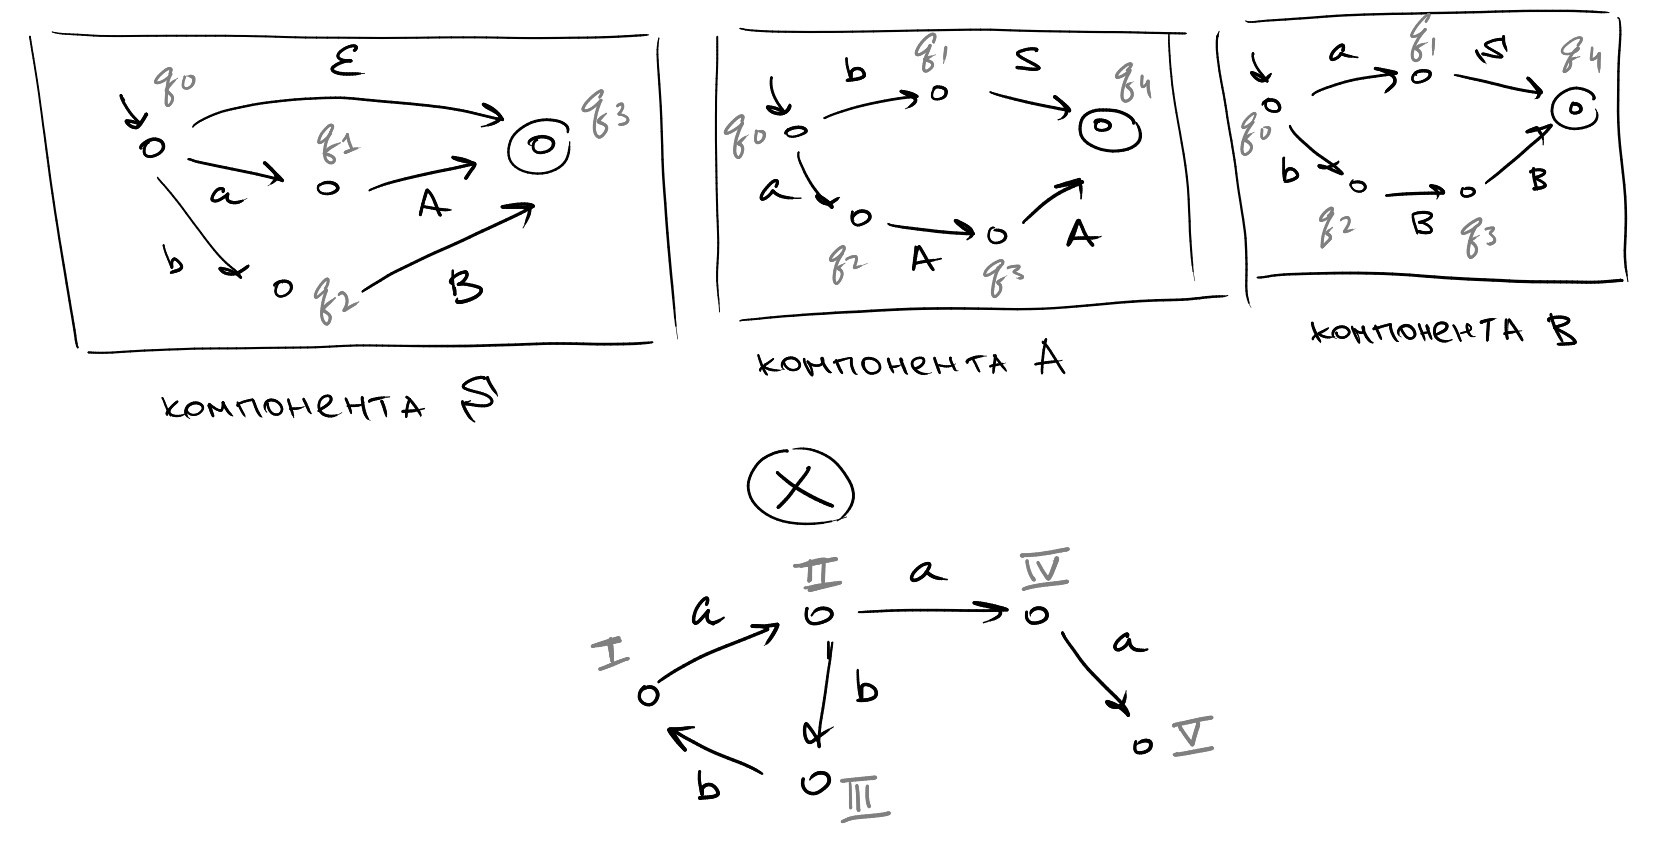
\includegraphics[width=1\linewidth]{img/example_intersection1.png}

        \TODO: дорисовать пример (а потом перерисовать)


    \end{example}

    Так что Алгоритм П можно описать так:
    \begin{enumerate}
        \item Построим прямое произведение входной грамматики $\cool{R}$ и входного графа $G$: $\cool{P} = \cool{R} \otimes G$.
        \item Решим задачу достижимости для полученного РКА $\cool{P}$
        \item Из вершины $u$ в вершину $v$ входного графа существует путь, выводимой входной грамматикой $\cool{G}$ $\EQ$ в $\cool{P}$ есть путь из стартового состояния $(q_0, u)$ в конечное состояние $(q_f, v)$
    \end{enumerate}

    Рассмотрим внимательнее второй пункт~--- задачу достижимости для РКА. В случае обычного автомата эта задача эквивалентна задаче построения транзитивного замыкания~\cite{Yannakakis1990}. В случае же РКА задача осложняется наличием рекурсивных вызовов, которые разрешаются итеративно. (??)

    В листинге~\ref{algo:P} приведён псевдокод Алгоритма П.

    \TODO: что-то написать про епс-переходы

    \begin{algorithm}[H]
        \floatname{algorithm}{Listing}
        \begin{algorithmic}[1]
        \caption{Алгоритм достижимости для РКА}
        \label{algo:P}
        \Function{RSMReachability}{$\cool{R}$}
            \State{$A \gets$ Adjacency matrix for $\cool{R}$}
            \While{$A$ is changing}
                \State{$A' \gets \textit{transitiveClosure}(A)$}
                \For{$i \in 1..k$}
                   \For{$u \in En_i$}
                        \For{$v \in Ex_i$}
                            \If{$A'_{u,v} \wedge \overline{A_{u,v}}$}
                                \State{$A' \gets A' \cup getEdges(i, u, v)$}
                            \EndIf
                        \EndFor
                   \EndFor
                \EndFor
                \State{$A \to A'$}
            \EndWhile
        \State \Return $A$
        \EndFunction
        \end{algorithmic}
    \end{algorithm}

    Работа происходит над матрицей смежности $\cool{R}$~--- изначально туда записываются все ``внутренние'' (нерекурсивные) рёбра. 

    Далее, внешний цикл повторяется, пока матрица смежности $A$ меняется (т.е. пока добавляются новые рёбра). На каждой итерации считается $A'$~--- транзитивное замыкание $A$. После этого находятся все новые пути вида $\langle$стартовое состояние$\rangle$ $\path$ $\langle$конечное состояние$\rangle$~--- те рёбра между стартовой и конечной вершинами компоненты, которых не было в $A$, но которые есть в $A'$~--- и добавляются соответствующие этим путям рёбра: для нового пути $(u \in En_i) \path (v \in Ex_i)$ проводятся все рёбра, соответствующие рекурсивным вызовам $i$-ой компоненты с начальной вершиной $u$ и конечной вершиной $v$.

\subsubsection{Алгоритм П2}

    Можно заметить, что не очень осмысленно на каждой итерации заново считать транзитивное замыкание, достаточно искать только пути, проходящие через рёбра, добавленные непосредственно на предыдущей итерации. То есть достаточно решать задачу {\bf инкрементального} транзитивного замыкания. 

    В листинге~\ref{algo:P2} приведён псевдокод Алгоритма П2 (основанного на инкрементальном ТЗ)

    \begin{algorithm}[H]
        \floatname{algorithm}{Listing}
        \begin{algorithmic}[1]
        \caption{Алгоритм достижимости для РКА (2)}
        \label{algo:P2}
        \Function{RSMReachability2}{$\cool{R}$}
            \State{$A \gets$ Empty adjacency matrix}
            \State{$Q \gets$ Empty Queue}
            \For{$i \in 1..k$}
                \For{$u \xrightarrow{c} v \in \delta_i$}
                    \State{$Q.Push(\langle u, v, i \rangle)$}
                \EndFor
            \EndFor
            \While{$Q$ is not Empty}
                \State{$\langle u, v, i \rangle \gets Q.Pop()$}
                \If{$u \in En_i \wedge v \in En_i$}
                    \Comment{Нашли новый путь}
                    \State{$A \gets A \cup getEdges(i, u, v)$}
                    \State{$Q.PushAll(getEdges(i, u, v))$}
                    \Comment{Добавляем новые рёбра}
                \EndIf
                \For{$x \in Q_i$}
                    \If{$A_{x, u} \wedge \overline{A_{x, v}}$}
                        \For{$y \in Q_i$} 
                            \If{$A_{v, y} \wedge \overline{A_{x, y}}$}
                                \State{$A \gets A \cup \langle x, y \rangle$}
                                \State{$Q.Push(\langle x, y, i \rangle)$}
                                \Comment{Обновлем транзитивное замыкание}
                            \EndIf
                        \EndFor
                    \EndIf
                \EndFor
            \EndWhile
        \State \Return $A$
        \EndFunction
        \end{algorithmic}
    \end{algorithm}

    В алгоритме используется (более менее) стандартная реализация инкрементального транзитивного замыкания~\cite{Ibaraki1983}. Для этого в ходе работы алгоритма поддерживается рабочая очередь $Q$ рёбер транзитивного замыкания, которые были найдены, но ещё не обработаны. 

    При обработке очередного \textit{(потому что оно из очереди ахахах)} ребра, ищутся новые пути, которые проходя через него. А именно, пусть было добавлено ребро $u \to v$. Тогда далее перебирается вершина $x$, такая что из неё была достижима вершина $u$ ($x \path u$), но не была достижима вершина $v$ ($x \not\path v$). Из такой вершины $x$ становятся достижимы все вершины $y$, которые были достижимы из $v$ ($v \path y$).

    Также, как и в Алгоритме П, если ребро ТЗ (= путь в графе) соединяет начальную и конечную вершину, в очередь добавляются также все соответствующие ему рекурсивные рёбра.

    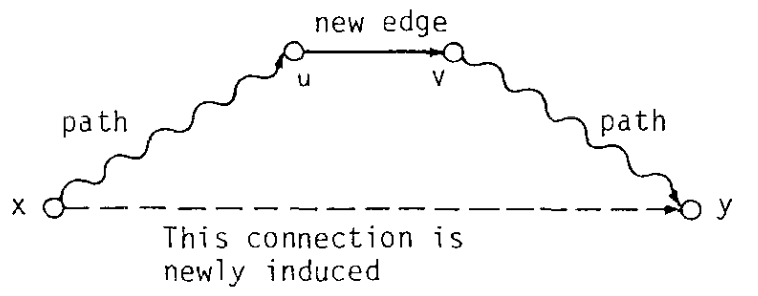
\includegraphics[width=1\linewidth]{img/TC_add.png}

    \TODO: норм картинка

    % Then algorithm iterates while matrix $M_2$ is changing. On each iteration the Kronecker product $M_3$ of matrices $M_1$ and $M_2$ is computed (that is adjacency matrix of Kronecker product $R \otimes \mathcal{G}$). After that, transitive closure $C_3$ of the product $M_3$ is computed. Then algorithm iterates over newly added edges (after transitive closure) and if one $(q_s, u) \rightsquigarrow (q_f, v)$ connects initial and final states of the same RSM box $S$, then new edge $u \xrightarrow{S} v$ is added. 
    
\subsection{Время работы}

\subsubsection{Алгоритм П}

\subsubsection{Алгоритм П2}

\subsection{Выводы и результаты по главе}
